\chapter{Kvalitetsarbete i praktiken}
\label{cha:indiv-report-wallstrom}
\chapterprecis{\LARGE{---- Fredrik Wallström ----}}


\section{Inledning}
\label{sec:introduction-wallstrom}

De flesta företag ute på marknaden idag strävar mot att utveckla bättre produkter, vassare tjänster och smidigare processer. Dessa produkter, tjänster och processer blir alltmer komplexa, samtidigt som företagen strävar efter att bli alltmer kostnadseffektiva. I arbetet med att utveckla nya produkter spelar kvalitetsarbetet en betydande roll. Det är ett problem att effektivisera kvalitetsarbetet för att hinna med dagens utveckling, då inte ens konsumenterna själva hinner med. Kvalitetssäkring är generellt ett komplext ämne att behandla, på grund av dess diffusa definition men det står klart att det är en viktig komponent i utvecklingen av dagens produkter, tjänster och processer.

\subsection{Syfte}
\label{sec:purpose-wallstrom}

Syftet med denna rapport är att ta reda på vad det innebär att kvalitetssäkra ett mjukvarusystem och vilka metoder det finns för ändamålet. Syftet är också att se över hur kvalitetsarbetet används i praktiken, samt om det finns möjligheter att utveckla och effektivisera detta arbete. Detta undersöks eftersom det blir alltmer aktuellt på grund av den snabba utvecklingen av produkter, tjänster och processer bland företagen i dagens samhälle.

\subsection{Frågeställning}
\label{sec:issue-wallstrom}

De frågeställningar som denna rapport kommer ta upp är:

\begin{enumerate}
	\item Vad är effekterna av att kvalitetssäkra mjukvaran för en produkt med den specifika metoden kodgranskning?
	\item Vad är de egentliga kostnaderna med att kvalitetssäkra en produkts mjukvara med kodgranskning, kommer effekterna för kvalitetssäkringen kompensera för den faktiska tidsåtgången?
\end{enumerate}

\clearpage

\section{Bakgrund}
\label{sec:background-wallstrom}
\subsection{Kvalitetssäkring}
Att säkerställa hög kvalité på ett system idag, innebär inte bara att testa och analysera systemet att det fungerar korrekt. För att försäkra sig själv och framförallt övertyga användaren om att systemet är i bra skick och presterar väl, kräver hög nogrannhet och disciplinerat kvalitetsarbete. Kvalitetssäkran är en process som genomförs kontinuerligt under uppbyggnaden av ett system och ingenting som appliceras vid systemet slutfas \cite{feldman2005quality}.

Att genomföra en kvalitetssäkrande process innebär enligt definiton, att tillhandahålla en försäkran om att programvaruprodukten och processer i produktens livscykel överensstämmer med deras specifika krav och håller fast vid de uppsatta planerna. \textit{Process}, är nyckelordet för kvalitetssäkran, det innebär alltså att kvalitetssäkran är en metod och inte en enstaka teknik. En annan viktig aspekt för kvalitetssäkran är att det inte behandlas som ett filosofiskt problem, utan mer som ett mätbart problem. Slutligen innebär kvalitetssäkran om att ge garantier och trovärdighet, produkten ska fungera rätt och folk ska tro att den fungerar rätt \cite{feldman2005quality}.

Kvalitetssäkran innefattar \textit{testning} som en av de viktigare aktiviteterna. Det finns dock ett ordspråk som säger att det inte går att testa kvaliten i produkten, utan att en testplan enbart kan fånga fel och ge ett mått på kvaliten. Det finns olika kvalitetssäkrande processer, de definieras för att passa behoven hos produkten. En process kan definieras för att försäkra sig om att designen är lämplig, implementationen är nogrann och att produkten möter alla krav innan publicering. Denna process kan även utvecklas till att analysera de upptäckta defekterna och sedan ständigt förbättra dessa \cite{feldman2005quality}.


\subsection{Kodgranskning}
Kodgranskning uppfattas som en effektiv process för att upptäcka fel och och fixa systemets defekter innan koden integreras med kodbasen \cite{mcintosh2014impact}. Denna process definierades av Fagan \cite{fagan1999design} och innebär att granskarna ska metodiskt följa checklistor för att sedan medverka i gruppmöten tillsammans med kodens författare. Kodgranskning har under åren moderniserats till att bli en flexibel lättviktsvariant av Fagans tidiga process. En modern kodgranskning består inte av checklistor eller personliga möten, utan den sker online. Idag finns det verktyg att ta hjälp av vid kodgranskning, bland annat har kodgranskning blivit starkt integrerat i olika versionshanteringsverktyg och problemhanteringssystem. Gerrit är ett exempel på ett väl använt och utvecklat verktyg för att underlätta kodgranskningsprocessen. Det finns alltså mycket som skiljer den moderna kodgranskningsprocessen med den som tillämpades förr, de båda har dock samma syfte, vilket är är att förbättra kvaliten på systemet \cite{shimagaki2016study}. 

Den generella processen för en modern kodgranskning kan sammafattas som följer. Först gör en utvecklare en ändring i koden och överlämnar den för granskning. I andra steget diskuterar andra utvecklare ändringarna och föreslår eventuella förbättringar i koden. Till sist accepterar en eller flera granskare ändringarna och koden integreras med källkoden \cite{kitagawa2016code}.

\subsection{Gerrit}
Gerrit är ett modernt kodgranskningsverktyg som underlättar en kodgranskningsprocess för ett git-baserat mjukvaruprojekt. Gerrit integrerar automatisk med testverktyg samt med kodverktyg. Metoden som används för att använda Gerrit är att författaren av koden laddar upp förslag på ändringar i systemet till en Gerrit server. Sedan kommer recensenter att evaluera koden och ge förslag på eventuella förbättringar. För att koden sedan ska godkännas kommer en kontrollant evaluera koden och verifiera dess korrekthet. Detta låter som en vanlig modern kodgranskningprocess men det som Gerrit underlättar med är det grafiska gränsnittet. Det hjälper till att få en överblick över statusen för de förslagna ändringarna. Gerrit ger också en möjlighet för teams att sätta olika krav och bekräftelse kriterier som krävs innan den förslagna ändringen integreras till källkoden \cite{mcintosh2014impact}.

\section{Teori}
\label{sec:theory-wallstrom}

Samhället idag ställer höga krav på tekniken. Eftersom dagens teknik i stor utsträckning består av produkter med ett integrerat system, innebär det att mjukvaruutvecklingen blir alltmer komplex. Mjukvaruutveckling består idag av en nogrann integrering av olika faktorer, som till exempel design, utveckling, användarvänlighet samt kompetenta programmerare med förmågan att sammarbeta. Det här innebär att idag läggs det alltmer vikt på att kvalitetsäkra ett mjukvarusystem för att tillfredsställa samhället. Oavsett hur avancerade verktyg, tekniker och metoder som har använts för att framställa en produkt är produkten oanvändbar om den inte gått igenom en kvalitetsäkrande process \cite{gill2005factors}.

Kodgranskning är en vanlig process för att öka kvaliten på koden och för att utsända kunskap inom projektet där koden är aktiv. McIntosh \cite{mcintosh2014impact} visar med en empirisk studie vilken påverkan en modern kodgranskningsprocess har på kvaliten hos ett mjukvarusystem. Denna empiriska studie har blivit möjlig att göra i modern tid eftersom det nu är möjligt att samla in hög kvalitativ data till studierna med hjälp av kodgranskningsverktyg, som tillexempel Gerrit. McIntosh analyserar huruvida det finns en relation mellan kodgranskning och kvalité genom att studera 3 stycken projekt. Studierna går ut på att undersöka hur kvaliten påverkas beroende på hur stor del av koden som har blivit kodgranskad samt hur många recensenter som deltagit i kodgranskningen. Det visar sig att både andelen kod granskad och hur många som har deltagit i kodgranskningen har en betydelsefull koppling till kvalité. Låg andel kod granskad samt lågt deltagande visar sig skapa mellan 2 till 5 stycken extra defekter efter produktlansering. McIntosh bekräftar med sin empiriska studie att dåligt granskad kod har negativa effekter på kvaliten på mjukvarusystem.

Vad är det då som gör att kodgranskning har blivit så viktigt för kvalitetssäkra ett mjukvarusystem? Beller \cite{beller2014modern} visar med en empirisk studie vad de praktiska fördelarna är med en modern kodgranskningsprocess. Med andra ord visar han vilka problem som löses med hjälp av denna process. Studien går ut på att manuellt klassificera 1400 ändringar som gjorts i en kodgranskningsprocess för öppen källkod. Beller kommer fram till att 7-35\% av de granskade kommentarerna kasseras samt att 10-22\% av ändringarna inte utlöstes av en kommentar ifrån kodgranskningen. Det uppstod även ett mönster i den granskade datan. Det visade sig att små uppgifter som till exempel bugg-fix, tenderar att ha mindre ändringar i en kommande kodgranskningsprocess än större uppgifter som involverar större kodkärna och implementationer av nya funktioner. Sammanfattningsvis visar Beller att majoriteten av ändringarna i en kodgranskningsprocess görs på grund av en granskares kommentar men det är även en hel del kommentarer som kasseras. Bellers slutsats är även att en homogen kodgranskning leder till samma antal ändringar i koden, oberoende på granskaren. Det är alltså typen av uppgifter som spelar roll, mindre uppgifter ger upphov till mindre ändringar och större uppgifter som involverar större kodkärna och fler filer, leder till fler ändringar.

\section{Metod}
\label{sec:method-wallstrom}

För att förstå effekterna av att genomföra en kodgranskningsprocess samt att inse vad de egentliga kostnaderna är med att kvalitetssäkra en produkt har en kvalitativ litteraturstudie genomförts. Litteraturstudien bestod av att analysera och bearbeta olika vetenskapliga rapporter som var relevant för ämnet ifråga. De utvalda rapporterna hade genomfört intressanta experiment och utredningar som kändes trovärdiga.

För att undersöka dessa frågor med en koppling till praktiken så har även ett praktiskt experiment gjorts på studenter ifrån Linköpings universitet. Dessa studenter har genomfört ett projekt där fokus var att leverera ett färdigt system med hög kvalité till kund. Experimentet bestod av att studenterna skulle svara på en enkät om hur det är att jobba med en kvalitetssäkrande process. Frågorna som studenterna fick svara på var följande:

\begin{itemize}
	\item Hur anser du det är att jobba med en kvalitetssäkrande process, är det positivt eller negativt, om man tar den faktiska tidsåtgången i åtanke?
	\item Har du jobbat med den specifika metoden kodgranskning för att säkerställa kvaliten på en produkt?
	\item Tycker du att kodgranskning hjälper att kvalitetssäkra en produkt?
	\item Anser du graden av deltagande människor i kodgranskningen hjälper eller försämrar kvaliten hos produkten? Blir det för komplicerat att anordna möten, tidsåtgången blir för stor, det tar för lång tid att få koden godkänd med mera.
	\item Har du några övriga tankar om att arbeta med en kvalitetssäkrande process eller med kodgranskning?
\end{itemize}

Detta experiment valdes eftersom att enbart utgå ifrån litteraturstudier inte ger en representativ bild av de relevanta kvalitetsfrågorna. Experimentets syfte är att se hur kvalitetsarbete fungerar i praktiken. Det är också intressant att se hur detta experiment skiljer sig ifrån resultatet av litteraturstudien. Det valdes studenter från Linköpings universitet eftersom det var viktigt att studenterna har jobbat med en kvalitetssäkrande process, vilket de har gjort under deras kandidatarbete. Det var också viktigt att studenterna hade en åsikt att förmedla vilket resulterar i bra underlag för hur det är att arbeta i en kvalitetssäkrande process. 

\section{Resultat}
\label{sec:results-wallstrom}

Resultaten ifrån den genomförda enkäten presenteras nedan:

\begin{itemize}
	\item \textbf{100\%} anser att det är positivt att jobba med en kvalitetsäkrande process.
	\item \textbf{88\%} har jobbat med den specifika metoden kodgranskningen för att säkerställa kvaliten på en produkt.
	\item \textbf{100\%} anser att kodgranskning hjälper till att kvalitetssäkra en produkt.
\end{itemize}
Figur G.1 nedan visar resultatet från frågan om graden av deltagande människor i en kodgranskningsprocess hjälper eller försämrar kvaliten hos en produkt.

\begin{figure}[H]
	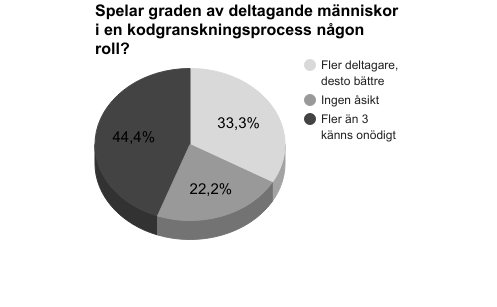
\includegraphics[width=100mm]{figures/grade_participation.png}
	\caption{Visar resultatet från om graden av deltagande människor i en kodgransningsprocess spelar någon roll.}
	\label{fig:grade_participation}
\end{figure}

\section{Diskussion}
\label{sec:discussion-wallstrom}
Resultatet av den genomförda enkäten visar att effekterna av en kodgranskningsprocess är positiva. 100\% anser att det är kodgranskning hjälper till att kvalitetssäkra en produkt. Det är endast få personer som inte använt sig av den specifika metoden kodgranskning för att kvalitetssäkra en produkt, utan istället använt sig av pargprogrammering vid utveckling av en produkt. Den här datan är inte tillräcklig och är en avgränsning i denna studie, för en mer representativ bild skulle det krävas större mängd data. 

Det intressanta med resultatet ifrån enkäten är att 44,4\% av de som deltog anser att om fler än 3 personer deltar i en kodgranskningsprocess finns det risk att tidsåtgången inte kompenserar för den faktiska vinsten med granskningen. Detta är också något som Beller \cite{beller2014modern} kommer fram till i sin studie angående vilka problem som löses med hjälp av kodgranskning. Beller anser att en homogen kodgranskning leder till samma antalet ändringar i koden, oberoende av vem som granskar. Det spelar alltså inte någon roll vem som granskar koden, den kommer heller inte blir bättre desto fler som granskar. Resultatet tyder alltså på att en kodgranskningsprocess inte bör innehålla fler deltagande personer än tre för att kvalitetssäkra produkten. 

Samtidigt visar McIntosh \cite{mcintosh2014impact} att kodgranskningsprocesser med lågt deltagande uppskattningsvis innehåller upp till 5 stycken defekter efter lansering, vilket kan låta som en kontradiktion till Bellers \cite{beller2014modern} resultat. McIntosh specificerar dock inte att det finns ett optimalt antal personer som ska delta i en kodgranskningsprocess för att göra den så effektiv och kvalitetssäkrande som möjligt. Den intressanta fråga som jag då ställer mig är om det finns ett optimalt antal deltagande personer i en kodgranskningsprocess? Det är en fråga som utifrån egna slutsatser inte finns något svar på. Det är en bred fråga och beror på hur stort projektet är och vad det finns för kvalitetsmål på produkten. Desto högre kvalitetsmål, desto fler personer bör delta i kodgranskningsprocesserna känns intuitivt som en bra approach. Denna studie visar dock att så inte är fallet, kodgranskningen riskerar bli ineffektiv vilket således kan leda till icke komplett produkt. Det här är en intressant frågeställning som kräver vidare efterforskning. Även här finns det såklart avgränsningar som bör tas med i åtanke. Dels innehåller inte enkäten tillräckligt med data och därtill skulle det även behövas göra en mer omfattande litteraturstudie för att få en representativ bild över situationen.

 

\section{Slutsatser}
\label{sec:conclusions-wallstrom}
Utifrån den genomförda enkäten men framförallt utifrån den gjorda literatustudien visar denna rapport att kvalité och kodgranskning har en stark relation. Att genomföra en kodgranskningsprocess visar sig tydligt ha positiva effekter på produktens kvalité. För att svara på fråga 1 i \eqref{sec:issue-wallstrom} så tyder resultatet från denna studie på att effekterna av en kodgranskningsprocess är positiva ur kvalitetssynpunkt. McIntosh \cite{mcintosh2014impact} visar att en dåligt granskad kod ger upphov till 2-5 stycken extra defekter efter produktlansering.

För att svara på fråga 2 i \eqref{sec:issue-wallstrom} så tyder resultatet från denna studie att kostnaden för en kodgranskningsprocess kompeserar för den faktiska tidsåtgången. Den genomförda enkäten visade att 100\% av deltagarna anser att kodgranskning hjälper till att kvalitetssäkra en produkt. Enkäten visar också att graden av deltagande människor i kodgranskningen inte behöver överstiga 3 stycken, detta kan leda till onödig tidsåtgång. Det här är även något som bekräftas av Bellers studie \cite{beller2014modern}. Slutsatsen av detta är att effekterna av en kodgranskningsprocess kompeserar den faktiska tidsåtgången så länge antalet personer som granskar inte överstigar 3 stycken.


%%%%%%%%%%%%%%%%%%%%%%%%%%%%%%%%%%%%%%%%%%%%%%%%%%%%%%%%%%%%%%%%%%%%%%
%%% person-report.tex ends here
